\chapter{Praktische Anwendung von SHAP auf lineare Modelle}

In diesem Kapitel wird der Einsatz des SHAP-Frameworks zur Interpretation linearer Modelle im 
Kontext des maschinellen Lernens untersucht. Lineare Modelle, gekennzeichnet durch ihre Transparenz 
und einfache Struktur, bilden oft die Basis für das Verständnis komplexerer Algorithmen. 
Dennoch bleibt die Herausforderung bestehen, die Beiträge individueller Merkmale zur Modellvorhersage zu 
quantifizieren und zu interpretieren.

Die Anwendung von SHAP-Werten ermöglicht es, diesen Herausforderungen zu begegnen und Einblicke in 
die Modellvorhersagen zu gewähren, die über traditionelle Methoden hinausgehen. 
Dieses Kapitel führt in die Grundlagen des \textsf{shap}-Pakets ein, demonstriert dessen Anwendung auf einen 
spezifischen Datensatz und diskutiert die Berechnung sowie Interpretation der resultierenden SHAP-Werte.

\section{Lineare Modelle als analytische Grundlage}

In linearen Regressionsmodellen wird die Zielgröße als eine gewichtete Kombination der Eingangsmerkmale bestimmt. 
Die einfache lineare Struktur dieser Modelle erleichtert das Verständnis der Beziehungen zwischen den Eingangsdaten 
und den Vorhersagen. 

Lineare Modelle sind ein grundlegendes Werkzeug in der statistischen Modellierung und dienen dazu, das Verhältnis zwischen 
einer abhängigen Variablen, die üblicherweise mit $y^{(i)}$ bezeichnet wird, 
und einem oder mehreren Prädiktoren, den unabhängigen Variablen $x_i$, zu erfassen. 
Diese Beziehungen werden mittels linearer Gleichungen dargestellt, die für jede 
einzelne Beobachtung $i$ im Datensatz folgendermaßen formuliert werden können:

\begin{equation}
    y^{(i)} = \beta_0 + \sum_{j=1}^{p} \beta_j x^{(i)}_j + \epsilon^{(i)},
\label{eq:reg-model}
\end{equation}

wobei das Ergebnis, das von einem linearen Modell für eine gegebene Beobachtung vorhergesagt wird, sich als Summe der mit 
Gewichten $\beta_j$ versehenen Merkmale $p$ ergibt.

Hierbei stellt $y^{(i)}$ den beobachteten Wert der abhängigen Variablen für die Beobachtungseinheit
$i$ dar. Der Term $\beta_0$ ist der Achsenabschnitt oder y-Achsenabschnitt des Modells, 
welcher den erwarteten Wert von $y$ darstellt, wenn alle unabhängigen Variablen $x$ null sind. 
Die Summe $\sum_{j=1}^{p} \beta_j x^{(i)}_j$ berechnet sich aus den Produkten der Koeffizienten 
$\beta_j$ und den Werten der unabhängigen Variablen $x^{(i)}_j$ für jede Beobachtungseinheit $i$ 
und jeden Prädiktor $j$, wobei die Koeffizienten $\beta_j$ den geschätzten Einfluss der 
entsprechenden unabhängigen Variablen auf die abhängige Variable beschreiben.

Der Fehlerterm $\epsilon^{(i)}$ steht für die Residuen, also die Differenzen zwischen den beobachteten 
und durch das Modell geschätzten Werten von $y^{(i)}$. Es wird angenommen, dass diese Fehler normalverteilt sind, 
was bedeutet, dass Abweichungen in beiden Richtungen um den Mittelwert (hier Null) 
mit abnehmender Wahrscheinlichkeit für größere Fehler auftreten \cite[S. 37]{Molnar_2022}.

In einem linearen Modell stellt der Achsenabschnitt die Basislinie dar, an der die Auswirkungen aller 
anderen Merkmale gemessen werden. Dieser Wert gibt an, was das Modell für die Zielvariable vorhersagen 
würde, wenn alle anderen Merkmale nicht vorhanden wären – der Ausgangspunkt der Vorhersage 
für einen Datensatz, in dem alle anderen Variablen auf null gesetzt sind. 
Es ist wichtig zu erwähnen, dass der Achsenabschnitt für sich genommen nicht immer eine praktische 
Bedeutung hat, da es selten vorkommt, dass alle Variablen tatsächlich den Wert null annehmen. 
Die wahre Aussagekraft des Achsenabschnitts tritt zutage, wenn die Daten so standardisiert wurden, 
dass ihre Mittelwerte bei null und die Standardabweichung bei eins liegen. Unter diesen Umständen repräsentiert der Achsenabschnitt 
die erwartete Zielvariable für einen hypothetischen Fall, in dem alle Merkmale ihren Durchschnittswert 
aufweisen.

Bei der Betrachtung einzelner Merkmale innerhalb des Modells sagt das Gewicht $\beta_j$ eines Merkmals, 
um wie viel sich die Zielvariable $y^{(i)}$ ändert, wenn das Merkmal $x^{(i)}_j$ um eine Einheit erhöht wird – und zwar unter 
der Annahme, dass alle anderen Merkmale unverändert bleiben. 
Dies ermöglicht es, den isolierten Effekt eines jeden Merkmals auf die Vorhersage zu verstehen \cite[S. 39]{Molnar_2022}.

Die optimalen Gewichte, oder Koeffizienten, eines linearen Regressionsmodells werden üblicherweise durch ein Verfahren bestimmt, 
das als Methode der kleinsten Quadrate (engl. \textit{Ordinary Least Squares}, OLS) bekannt ist. 
Diese Methode sucht die Koeffizienten \( \beta_0, \ldots, \beta_p \), welche die Summe der quadrierten 
Differenzen zwischen den beobachteten Werten der Zielvariablen \( y^{(i)} \) und den von dem Modell 
vorhergesagten Werten minimieren:

\begin{equation}
    \hat{\beta} = \arg \underset{\beta_0, \ldots, \beta_p}{\min} \ \sum_{i=1}^{n} \left( y^{(i)} - \left( \beta_0 + \sum_{j=1}^{p} \beta_j x_j^{(i)}\right)\right)^2.
\end{equation}

Das Ergebnis der Minimierung, \( \hat{\beta} \) stellt den Vektor der geschätzten Koeffizienten dar \cite[S. 37]{Molnar_2022}. 
In der vorliegenden Arbeit wird das Python-Paket \textsf{scikit-learn}\footnote{\url{https://scikit-learn.org}} verwendet, um die lineare Regression durchzuführen und die Koeffizienten 
\( \hat{\beta} \) zu bestimmen. 


\section{Einführung in das \textsf{shap} Python-Paket}
\label{sec:shap-package}

Das Python-Paket \textsf{shap}\footnote{\url{https://shap.readthedocs.io}} ist eine Open-Source-Bibliothek, die es Nutzern ermöglicht, 
die Auswirkungen von Merkmalen auf Vorhersagen von maschinellen Lernmodellen zu interpretieren und zu visualisieren. 
Entwickelt wurde die Bibliothek ursprünglich von Scott Lundberg und weiteren Mitwirkenden im Rahmen der Forschungsarbeit 
an der University of Washington \cite{NIPS2017_8a20a862}. Das Paket basiert auf dem Konzept der Shapley-Werte aus der kooperativen Spieltheorie 
und überträgt diese auf den Kontext des maschinellen Lernens, um als Tool für die Interpretierbarkeit und Erklärbarkeit 
von Modellvorhersagen zu dienen.

\urldef{\ploturl}\url{https://shap.readthedocs.io/en/latest/api.html#plots}

Die Kernfunktion des \textsf{shap}-Pakets ist die Berechnung von SHAP-Werten, welche die Auswirkung der 
Einzelmerkmale auf die Modellvorhersage quantifizieren. Jeder SHAP-Wert ist ein Maß dafür, wie viel jedes Merkmal 
zur Vorhersage beigetragen hat, im Vergleich zu einer durchschnittlichen Vorhersage über den gesamten Datensatz. 
Diese Werte sind besonders wertvoll, weil sie ein Maß für die Bedeutung jedes Merkmals liefern, 
das sowohl lokal (für einzelne Vorhersagen) als auch global (über das gesamte Modell) interpretiert werden kann.

Mit \textsf{shap} können Benutzer die Vorhersagen einer Vielzahl von Modellen interpretieren, 
von linearen Modellen bis hin zu komplexen Konstrukten wie tiefe neuronale Netzwerke. 
Die Bibliothek bietet eine vielseitige Auswahl an Visualisierungsoptionen, darunter Beeswarm-Plots, Dependence-Plots und 
Bar-Plots, die es ermöglichen, die SHAP-Werte intuitiv zu verstehen. Eine Übersicht aller Visualisierungsoptionen ist in der Dokumentation 
des Pakets zu finden\footnote{\ploturl}.
Diese Visualisierungen erleichtern es, Muster und Beiträge einzelner Merkmale zu erkennen, 
was nicht nur wertvolle Einblicke in die Leistung des Modells bietet, sondern auch zu faireren und transparenteren 
Modellentscheidungen führen kann. 

\urldef{\shapurl}\url{https://shap.readthedocs.io/en/latest/api.html#explainers}
\urldef{\exacturl}\url{https://github.com/shap/shap/blob/master/shap/explainers/_exact.py}

Im Kapitel \ref{subsec:linear-shap-estimator} wurde bereits der LinearExplainer aus dem \textsf{shap}-Paket 
vorgestellt, ein Beispiel für die verschiedenen Estimators, die das Paket in Form von Explainern bereitstellt. 
Das Paket bietet eine Vielzahl von Explainern, die auf unterschiedliche Modelltypen zugeschnitten sind. 
Einer der bemerkenswerten Aspekte von \textsf{shap} ist der auto Modus des Estimators, 
der automatisch den am besten geeigneten Explainer für das gegebene Modell auswählt. 
Diese Funktion ist besonders nützlich, da sie die Komplexität der Auswahl des richtigen Explainers 
reduziert und den Anwendungsprozess vereinfacht. Speziell für Modelle mit ca. 15 Merkmalen\footnote{\exacturl} wählt der 
auto Modus den exakten Explainer, der präzise SHAP-Werte auf Grundlage aller Daten und Koalitionen berechnet, was für Modelle mit einer geringeren Anzahl 
von Merkmalen effizient und praktikabel ist \cite[S. 40f]{Molnar_2023}. Eine Übersicht der zur Verfügung stehenden \textsf{shap}-Explainern ist in der
Dokumentation des Pakets zu finden\footnote{\shapurl}. 


\section{Einführung in den Datensatz}

In der vorliegenden Arbeit wird der SGEMM GPU Kernel Performance Datensatz verwendet, welcher die Laufzeitmessung eines Matrix-Matrix-Produkts 
\(A*B = C\) dokumentiert, wobei alle Matrizen die Größe 2048 x 2048 haben. 
Der Datensatz wurde erstellt, um verschiedene Konfigurationen eines parameterisierbaren SGEMM 
(Single-precision General Matrix Multiply) GPU-Kernels zu testen. Mit insgesamt 261400 möglichen Parameterkombinationen, 
von denen jede viermal ausgeführt wurde, bietet der Datensatz eine umfassende Grundlage zur Untersuchung der Laufzeitperformance.
Die Daten wurden von Enrique G. Paredes und Rafael Ballester-Ripoll vom Visualization and MultiMedia Lab der Universität 
Zürich gesammelt \cite{ballesterripoll2017sobol, Nugteren_2015}. 

Der Datensatz umfasst folgende Variablen \cite{misc_sgemm_gpu_kernel_performance_440}:

\begin{itemize}
    \item \textbf{MWG, NWG} (Matrix Widths for Global tile size): Dimensionen der 2D-Aufteilung einer Matrix auf Workgroup-Ebene. Mögliche Werte sind \{16, 32, 64, 128\}, was die Anzahl der Datenpunkte in jeder Dimension angibt.
    \item \textbf{KWG} (Kernel Width for Global tile size): Innere Dimension der 2D-Aufteilung auf Workgroup-Ebene. Mögliche Werte sind \{16, 32\}, ebenfalls als Anzahl der Datenpunkte.
    \item \textbf{MDIMC, NDIMC} (Local Workgroup Size): Dimensionen für die lokale Workgroup-Größe. Werte in \{8, 16, 32\}, repräsentieren die Anzahl der Threads pro Dimension innerhalb einer Workgroup.
    \item \textbf{MDIMA, NDIMB} (Local Memory Shape): Dimensionen, die die Form des lokalen Speichers bestimmen. Werte sind \{8, 16, 32\} und beziehen sich auf die Größe des Speicherblocks pro Dimension.
    \item \textbf{KWI} (Kernel Workgroup unrolling): Ein Faktor für das Kernel Loop Unrolling. Mögliche Werte sind \{2, 8\}, die den Grad der Schleifenvereinfachung angeben.
    \item \textbf{VWM, VWN} (Vector Widths for loading/storing): Vektorbreiten für das Laden und Speichern von Matrizen. Werte in \{1, 2, 4, 8\} repräsentieren die Anzahl der Datenpunkte, die simultan pro Operation gehandhabt werden.
    \item \textbf{STRM, STRN} (Enable stride): Binäre Einstellungen, die festlegen, ob ein Stride für den Speicherzugriff innerhalb eines Threads aktiviert ist. Werte \{0, 1\} repräsentieren ausgeschaltet bzw. eingeschaltet.
    \item \textbf{SA, SB} (Manual Caching): Binäre Variablen zur Aktivierung der manuellen Zwischenspeicherung von 2D Workgroup-Kacheln. Werte \{0, 1\} repräsentieren ausgeschaltet bzw. eingeschaltet.
    \item \textbf{Run1, Run2, Run3, Run4} (Performance Times): Vier unabhängige Laufzeiten (in Millisekunden) für jede Parameterkombination. Sie zeigen die Performanz des GPU-Kernels unter verschiedenen Einstellungen und Bedingungen. Die Zeiten variieren zwischen 13.25 ms und 3397.08 ms.
\end{itemize}

\section{Explorative Datenanalyse \& Datenaufbereitung}

Der Datensatz wurde in Python mithilfe der Bibliothek \textsf{pandas} als \textsf{Dataframe} eingelesen.
Die Zielvariable Runtime für die Regression wurde als Durchschnitt der vier unabhängigen Laufzeiten (Run1, Run2, Run3 und Run4) berechnet, 
um eine repräsentative Maßzahl für die Gesamtperformance zu erhalten.

Der vollständige Quellcode für das Einlesen der Daten sowie alle weiteren Analyseschritte ist 
im Anhang \ref{linreg} dieser Arbeit zu finden.

Tabelle \ref{tab:df-head} zeigt die ersten fünf Beobachtungen des Datensatzes:

\begin{table}[!h]
    \caption{Auszug aus dem SGEMM GPU Kernel Performance Datensatz.}
    \footnotesize
    \begin{tabularx}{\textwidth}{Xrrrrrrrrrrrrrrr}
    \toprule
    Index & \rotatebox{90}{MWG} & \rotatebox{90}{NWG} & \rotatebox{90}{KWG} & \rotatebox{90}{MDIMC} & \rotatebox{90}{NDIMC} & \rotatebox{90}{MDIMA} & \rotatebox{90}{NDIMB} & \rotatebox{90}{KWI} & \rotatebox{90}{VWM} & \rotatebox{90}{VWN} & \rotatebox{90}{STRM} & \rotatebox{90}{STRN} & \rotatebox{90}{SA} & \rotatebox{90}{SB} & \rotatebox{90}{$\varnothing$ Runtime (ms)} \\
    \midrule
    0 & 16 & 16 & 16 & 8 & 8 & 8 & 8 & 2 & 1 & 1 & 0 & 0 & 0 & 0 & 116.3700 \\
    1 & 16 & 16 & 16 & 8 & 8 & 8 & 8 & 2 & 1 & 1 & 0 & 0 & 0 & 1 & 78.7050 \\
    2 & 16 & 16 & 16 & 8 & 8 & 8 & 8 & 2 & 1 & 1 & 0 & 0 & 1 & 0 & 80.5650 \\
    3 & 16 & 16 & 16 & 8 & 8 & 8 & 8 & 2 & 1 & 1 & 0 & 0 & 1 & 1 & 86.6375 \\
    4 & 16 & 16 & 16 & 8 & 8 & 8 & 8 & 2 & 1 & 1 & 0 & 1 & 0 & 0 & 118.6625 \\
    \bottomrule
    \end{tabularx}
    \label{tab:df-head}
    \normalsize\\
    Quelle: Eigene Darstellung auf Basis der Datengrundlage \cite{misc_sgemm_gpu_kernel_performance_440}.
\end{table}

In Tabelle \ref{tab:statistics} sind deskriptive Statistiken der verschiedenen Variablen des Datensatzes dargestellt. 

\begin{table}[!h]
    \caption{Auszug aus dem SGEMM GPU Kernel Performance Datensatz.}
    \footnotesize
    \begin{tabularx}{\textwidth}{Xrrrrrrr}
    \toprule
    Variable & mean & std & min & 25\% & 50\% & 75\% & max \\
    \midrule
    MWG & 80.415364 & 42.469220 & 16.0000 & 32.0000 & 64.00 & 128.0000 & 128.0000 \\
    NWG & 80.415364 & 42.469220 & 16.0000 & 32.0000 & 64.00 & 128.0000 & 128.0000 \\
    KWG & 25.513113 & 7.855619 & 16.0000 & 16.0000 & 32.00 & 32.0000 & 32.0000 \\
    MDIMC & 13.935894 & 7.873662 & 8.0000 & 8.0000 & 8.00 & 16.0000 & 32.0000 \\
    NDIMC & 13.935894 & 7.873662 & 8.0000 & 8.0000 & 8.00 & 16.0000 & 32.0000 \\
    MDIMA & 17.371126 & 9.389418 & 8.0000 & 8.0000 & 16.00 & 32.0000 & 32.0000 \\
    NDIMB & 17.371126 & 9.389418 & 8.0000 & 8.0000 & 16.00 & 32.0000 & 32.0000 \\
    KWI & 5.000000 & 3.000006 & 2.0000 & 2.0000 & 5.00 & 8.0000 & 8.0000 \\
    VWM & 2.448609 & 1.953759 & 1.0000 & 1.0000 & 2.00 & 4.0000 & 8.0000 \\
    VWN & 2.448609 & 1.953759 & 1.0000 & 1.0000 & 2.00 & 4.0000 & 8.0000 \\
    STRM & 0.500000 & 0.500001 & 0.0000 & 0.0000 & 0.50 & 1.0000 & 1.0000 \\
    STRN & 0.500000 & 0.500001 & 0.0000 & 0.0000 & 0.50 & 1.0000 & 1.0000 \\
    SA & 0.500000 & 0.500001 & 0.0000 & 0.0000 & 0.50 & 1.0000 & 1.0000 \\
    SB & 0.500000 & 0.500001 & 0.0000 & 0.0000 & 0.50 & 1.0000 & 1.0000 \\
    Runtime & 217.571953 & 368.750161 & 13.3175 & 40.6675 & 69.79 & 228.3875 & 3341.5075 \\
    \bottomrule
    \end{tabularx}
    \label{tab:statistics}
    \normalsize
    \\ Quelle: Eigene Darstellung, \ref{linreg}.
\end{table}

Die Zielvariable Runtime weist eine erhebliche Variabilität und Spannweite auf. 
Um eine homogenere Verteilung für die Regression zu erreichen und den Einfluss 
von Ausreißern zu verringern, wurde sie einer logarithmischen Transformation unterzogen, 
wie auch von den Datensatzautoren empfohlen \cite{misc_sgemm_gpu_kernel_performance_440}. 
Grafik \ref{pic:box} illustriert die Verteilungen der Runtime mittels Boxplots und Histogrammen, 
vor und nach der log-Transformation, und verdeutlicht den Effekt der Normalisierung:

\begin{figure}[!h]
    \caption{Verteilungen der Runtime vor und nach log-Transformation.}
    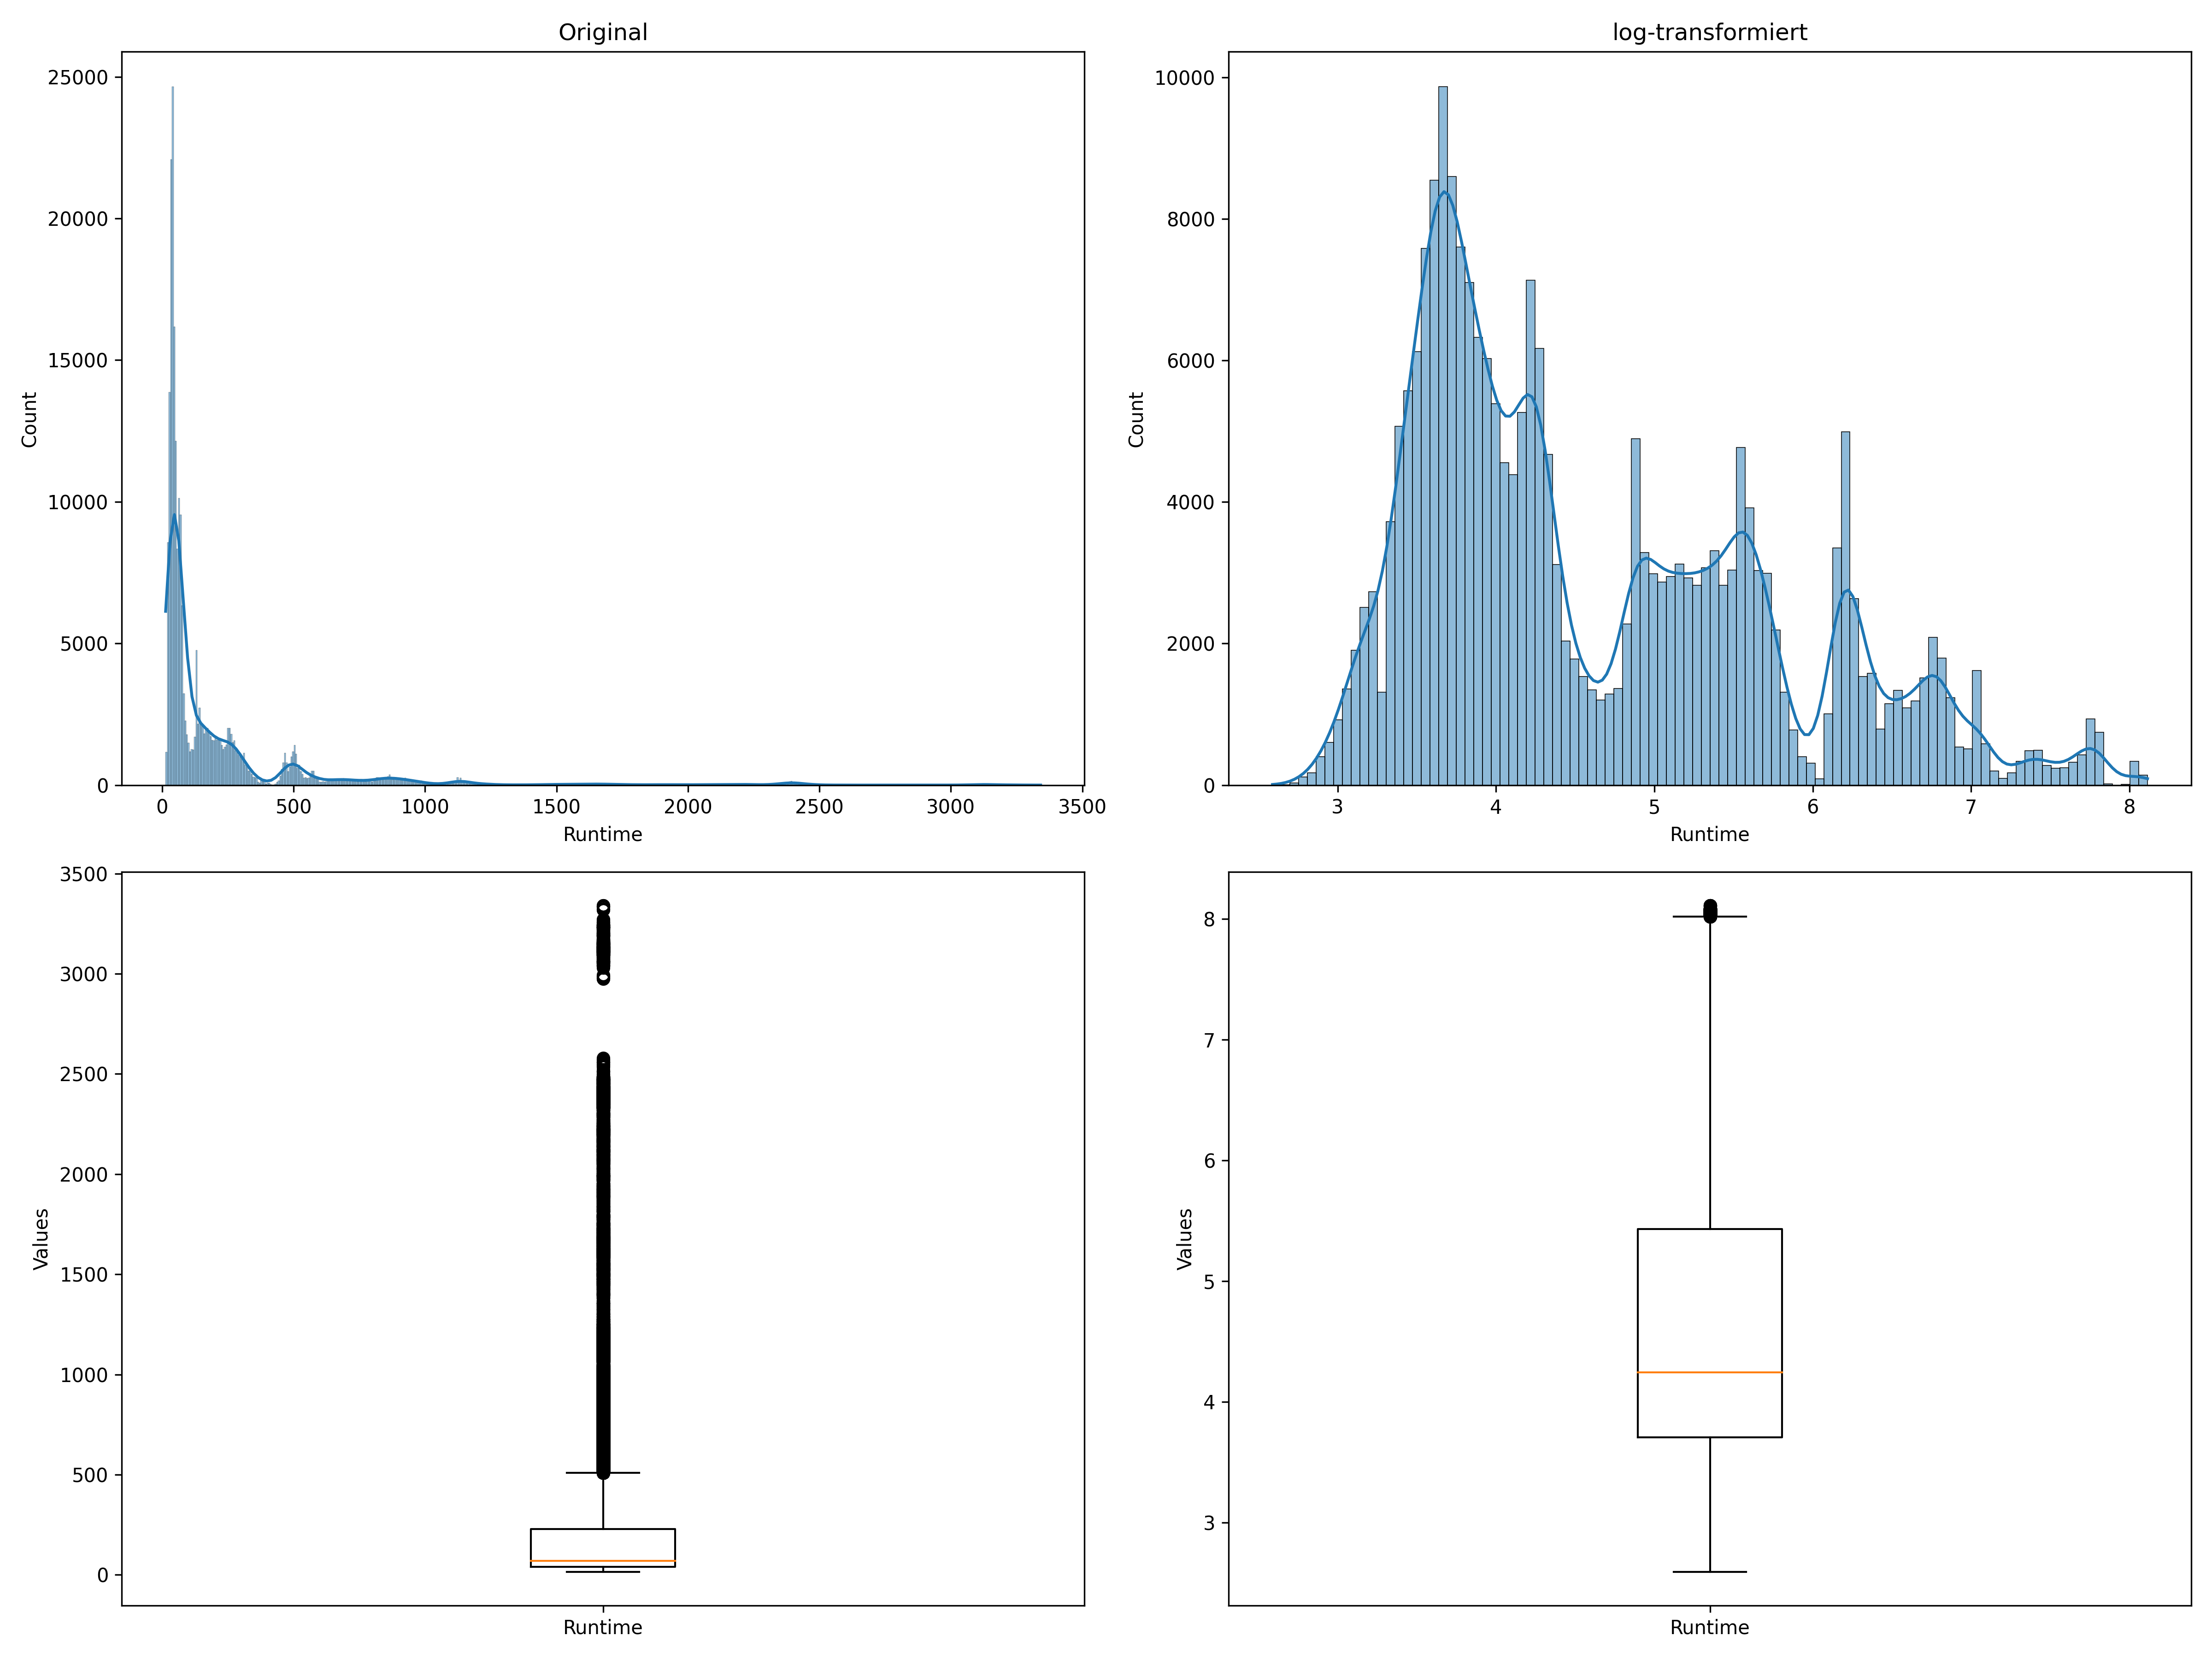
\includegraphics[width=1\textwidth]{../scripts/images/combined_runtime_plots.png}
    Quelle: Eigene Darstellung auf Basis der Datengrundlage \cite{misc_sgemm_gpu_kernel_performance_440}, \ref{linreg}.
    \label{pic:box}
\end{figure}

Abbildung \ref{pic:hist} zeigt die Verteilung aller Merkmale des Datensatzes. 

\begin{figure}[!h]
    \caption{Verteilungen der Merkmale.}
    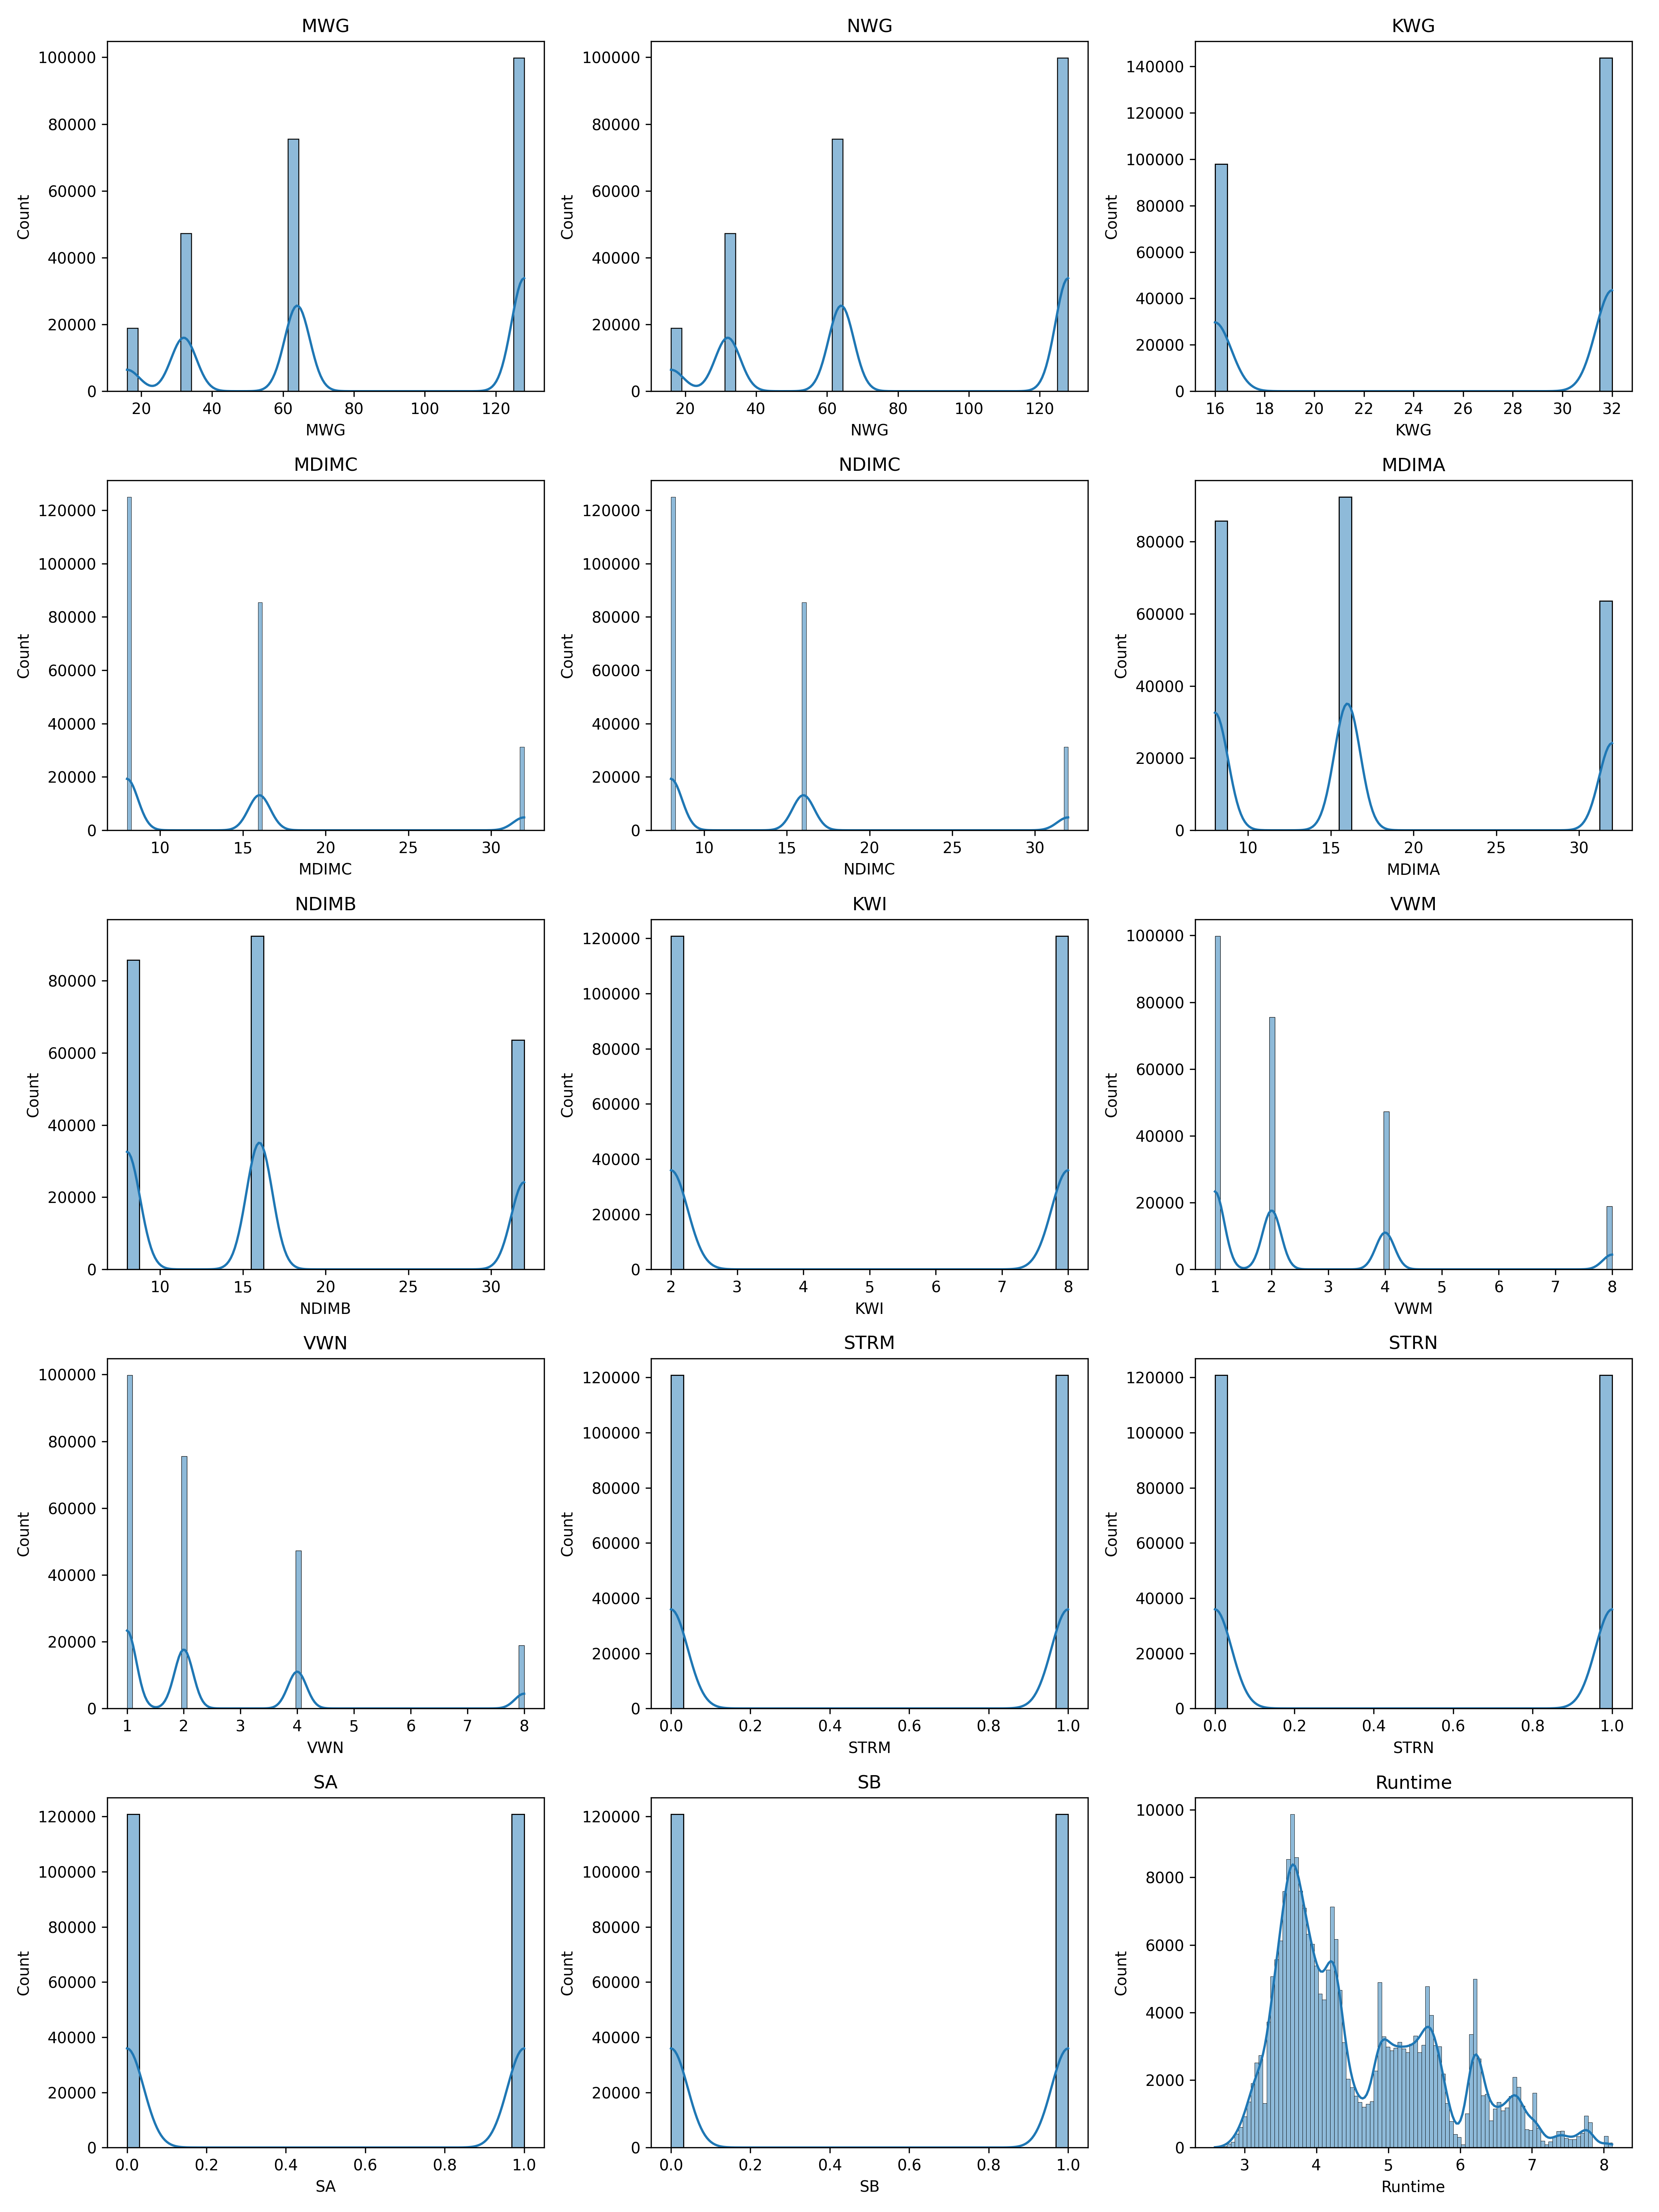
\includegraphics[width=1\textwidth]{../scripts/images/dist_gpu.png}
    Quelle: Eigene Darstellung auf Basis der Datengrundlage \cite{misc_sgemm_gpu_kernel_performance_440}, \ref{linreg}.
    \label{pic:hist}
\end{figure}

Die Korrelationsmatrix, die in Abbildung \ref{pic:corr} dargestellt ist, 
umfasst die Zielvariable Runtime, wodurch direkte Einblicke in die Beziehungen 
zwischen den Merkmalen und der Zielvariablen möglich sind. Die Koeffizienten variieren 
von -0.25 bis 0.46, was darauf hindeutet, dass einige Variablen eine moderate 
Korrelation mit der Runtime aufweisen. Positive Werte, wie der höchste Koeffizient 
von 0.46, implizieren, dass eine Erhöhung der entsprechenden Merkmalsausprägungen tendenziell 
mit längeren Ausführungszeiten verbunden ist. Negative Werte, wie der niedrigste Koeffizient 
von -0.25, deuten hingegen auf eine umgekehrte Beziehung hin, 
bei der höhere Merkmalsausprägungen mit kürzeren Laufzeiten korrelieren. 
Diese Korrelationen liefern wichtige Informationen für die Modellierung, da sie aufzeigen, 
welche Parameter möglicherweise einen stärkeren Einfluss auf die Laufzeit haben. 

\begin{figure}[!h]
    \caption{Korrelationsmatrix der Merkmale im Datensatz.}
    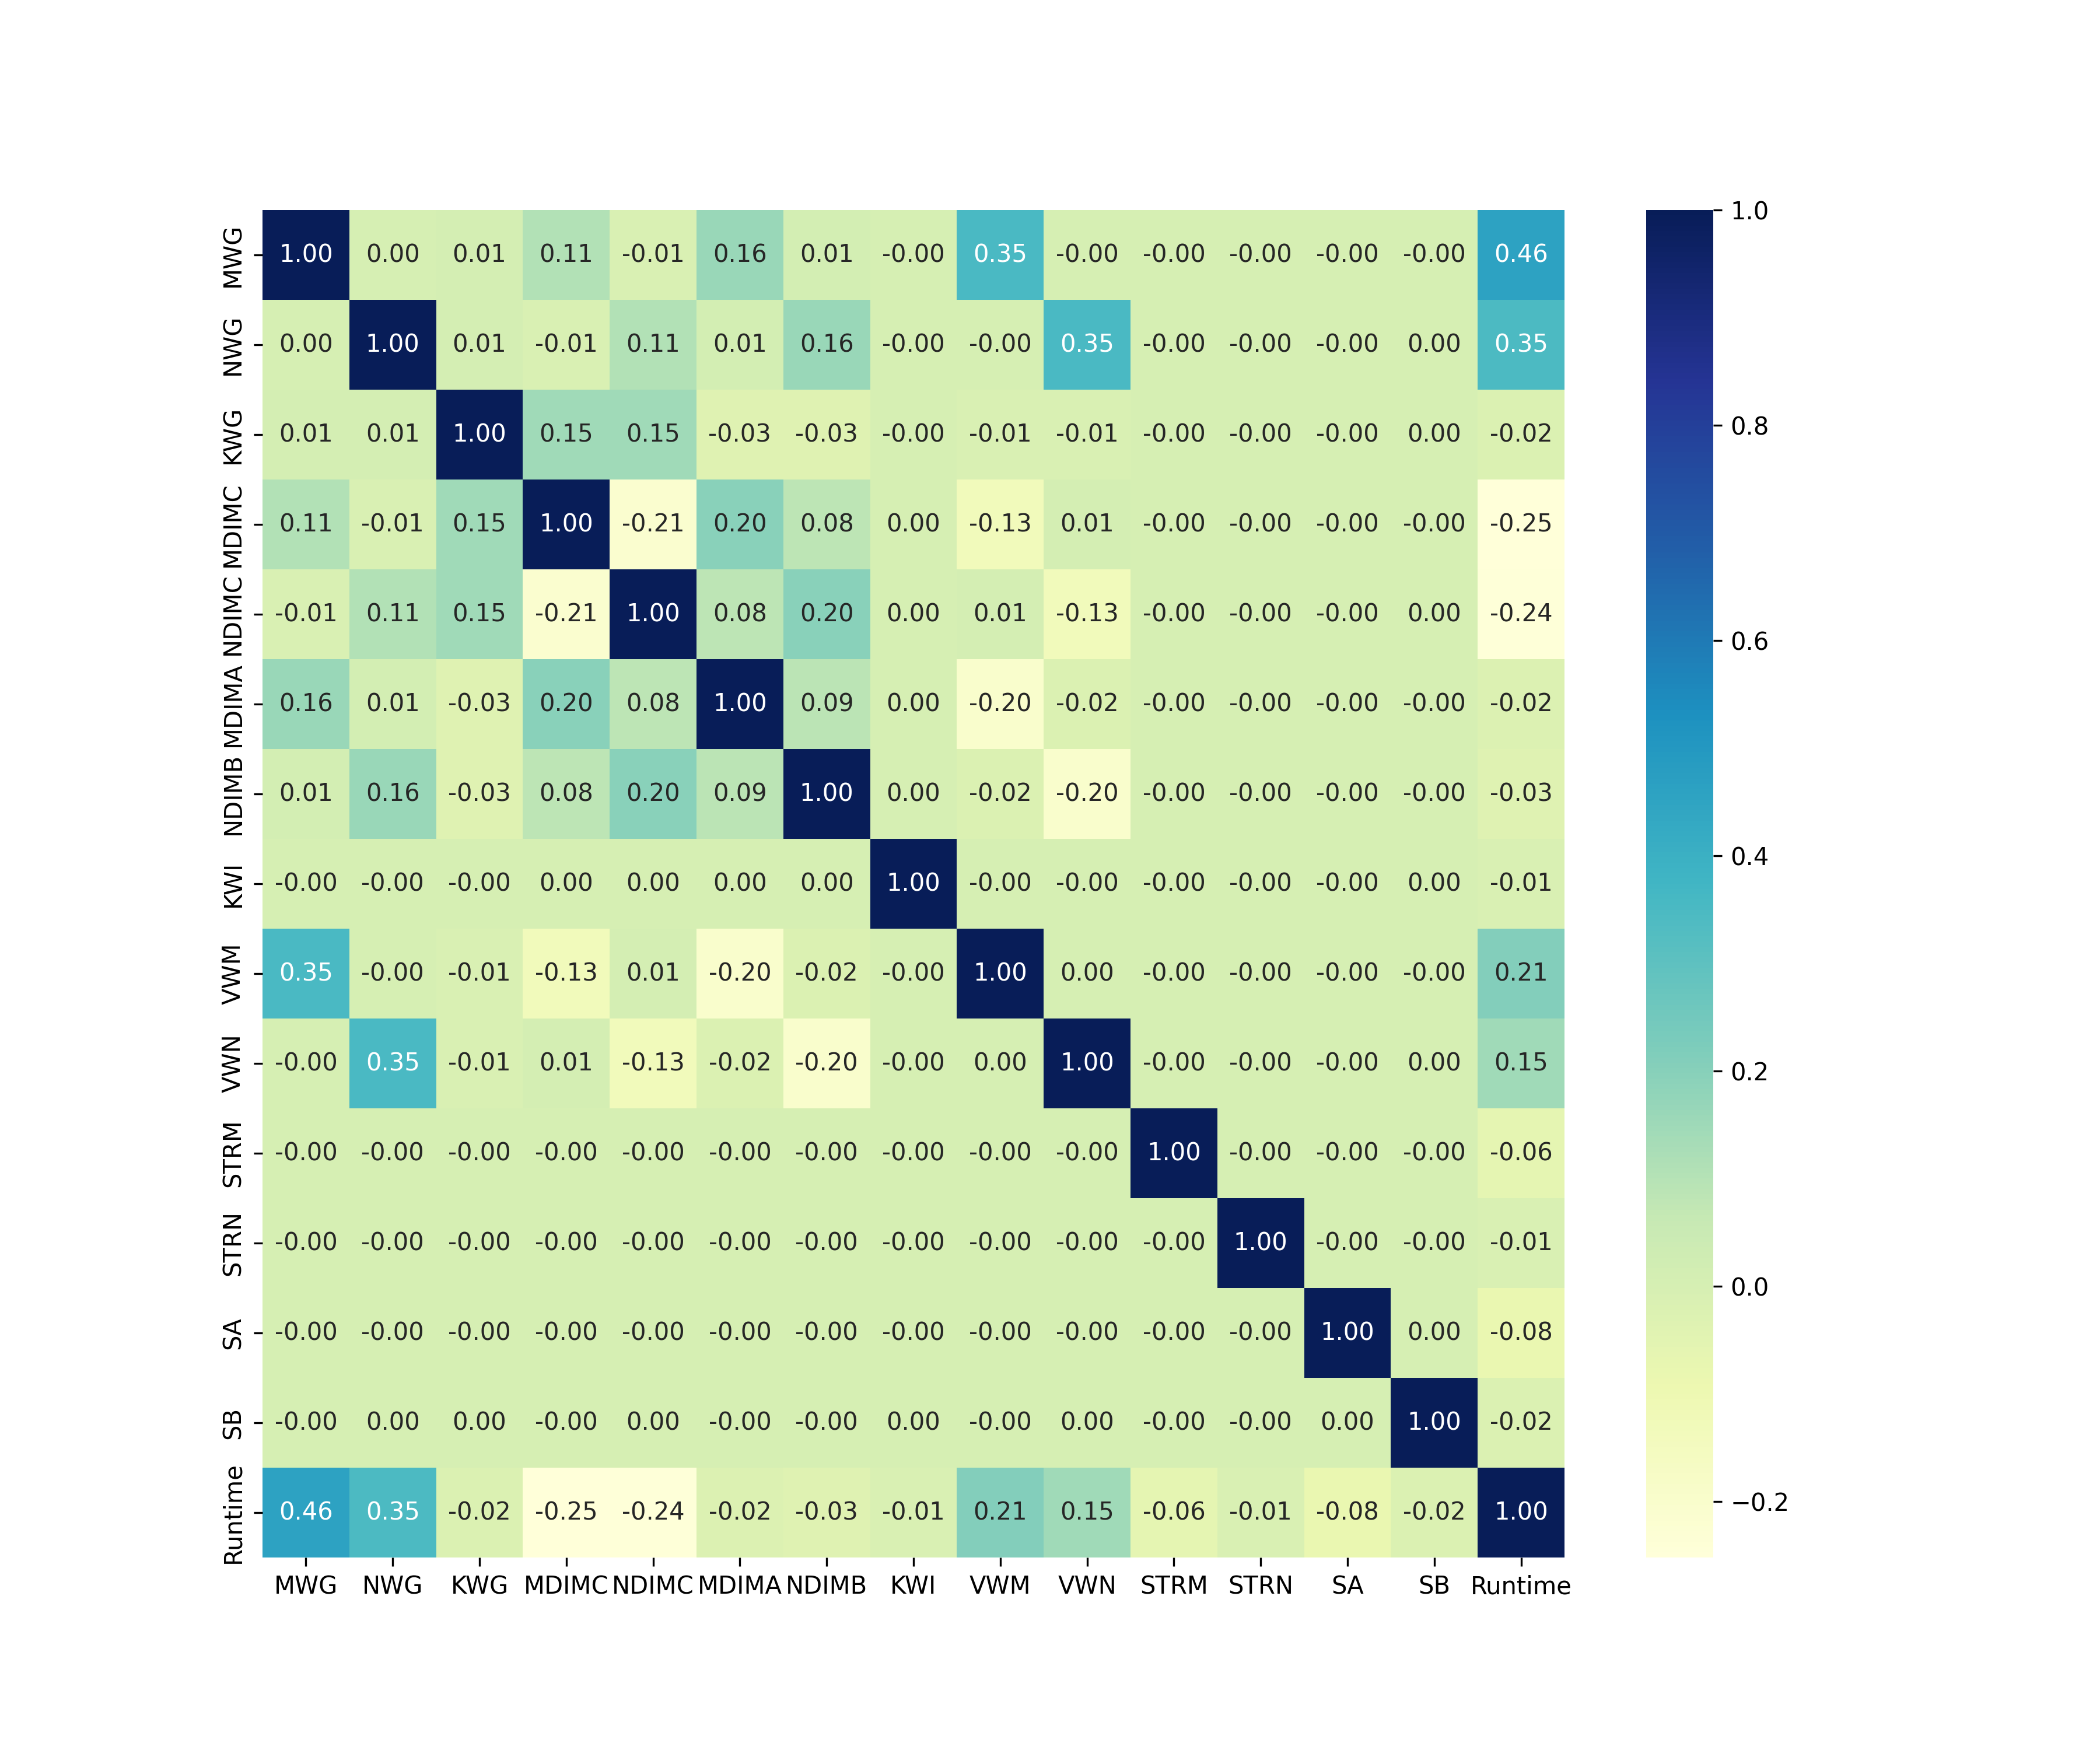
\includegraphics[width=1\textwidth]{../scripts/images/corr_gpu.png}
    Quelle: Eigene Darstellung, \ref{linreg}.
    \label{pic:corr}
\end{figure}

\section{Modellierung der linearen Regression}

Um die Beziehung zwischen den unabhängigen Variablen und der Zielvariablen 
Runtime zu untersuchen, wurde ein lineares Regressionsmodell aufgestellt. 
Zur Bewertung der Vorhersageleistung des Modells und zur Vermeidung von Overfitting wurde der 
Datensatz in zwei Teile aufgeteilt: 80\% der Daten dienten als Trainingsset zur 
Anpassung des Modells, während die restlichen 20\% als Testset verwendet wurden, 
um die Modellleistung anhand neuer, unbekannter Daten zu evaluieren. 
Diese Aufteilung erfolgte zufällig, aber reproduzierbar, durch Festlegen eines Seed-Werts 
für den Zufallszahlengenerator, der eine konsistente Teilung des Datensatzes ermöglicht.

Das Trainingsset wurde dazu verwendet, die Koeffizienten der linearen Regression zu schätzen, 
die den Einfluss jeder unabhängigen Variablen auf die Zielvariable quantifizieren. 
Anschließend wurde das Modell mit dem Testset geprüft, um seine Vorhersagegenauigkeit zu bewerten. 
Die Leistung des Modells wurde anhand von Metriken wie dem mittleren quadratischen Fehler (Mean Squared Error, MSE) gemessen, 
die ein Maß für die Abweichung der Modellvorhersagen von den tatsächlichen Werten darstellen.

Codeauschnitt \ref{code:model} und \ref{code:model-train} zeigen das Trainieren und Testen der zugrundeliegenden Daten 
eines linearen Regressionsmodells:

\lstinputlisting[language=Python,label=code:model, firstline=34, lastline=52, 
    caption={Initialisierung eines linearen Regressionsmodells, \ref{linreg}.}, captionpos=top]{../scripts/linreg.py}


\lstinputlisting[language=Python,label=code:model-train, firstline=183, lastline=190, 
    caption={Training und Testen eines linearen Regressionsmodells, \ref{linreg}.}, captionpos=top]{../scripts/linreg.py}


\section{Berechnung von SHAP-Werten}

Um SHAP-Werte zu berechnen, wird zunächst ein SHAP-Explainer-Objekt erstellt. In diesem Fall wird der Explainer 
von SHAP mit dem trainierten linearen Regressionsmodell und dem Trainingsdatensatz initialisiert. 
Anschließend werden die SHAP-Werte für die Testdaten berechnet, um die Beiträge der einzelnen Merkmale 
zu analysieren. Der Typ des Explainers wird durch die Art des übergebenen Modells bestimmt. 
Da in diesem Beispiel ein lineares Modell verwendet wird, wird automatisch ein geeigneter Explainer 
für lineare Modelle ausgewählt.

Das folgende Codeausschnitt \ref{code:shap} zeigt die Initialisierung des SHAP-Explainers und die Berechnung der SHAP-Werte:

\lstinputlisting[language=Python,label=code:shap, firstline=191, lastline=193, 
    caption={Berechnung von SHAP-Werten für das lineare Regressionsmodell, \ref{linreg}.}, captionpos=top]{../scripts/linreg.py}

Das Explainer-Objekt enthält neben den SHAP-Werten (.values), 
die die Einflüsse der einzelnen Merkmale der Testmenge auf die Modellvorhersage quantifizieren, 
auch die Basiswerte (.base\_values), die die durchschnittliche Vorhersage des Modells darstellen, 
und die ursprünglichen Merkmalsausprägungen (.data), die für die Berechnung dieser Werte verwendet wurden \cite[S. 51]{Molnar_2023}.

Dies bildet die Grundlage für den nächsten entscheidenden Schritt: 
die Visualisierung und tiefere Analyse dieser Werte. Die SHAP-Bibliothek bietet eine 
Reihe von leistungsstarken Visualisierungswerkzeugen, die es ermöglichen, die Auswirkungen 
der einzelnen Merkmale auf die Modellvorhersagen intuitiv und verständlich darzustellen. 

Im folgenden Kapitel \ref{chapter:results} werden diese Visualisierungen im Detail vorgestellt. 
Anhand von Beeswarm-Plots, Dependence-Plots und Bar-Plots werden die Ergebnisse der 
SHAP-Analyse dargestellt, die ein umfassendes Bild der Einflüsse und Wichtigkeiten der 
verschiedenen Merkmale im Kontext des linearen Regressionsmodells bieten.

Die Grafiken wurden mithilfe der \textsf{shap}-Bibliothek wie folgt erzeugt:

\lstinputlisting[language=Python,label=code:img, firstline=92, lastline=113, 
    caption={Erzeugen der SHAP Plots, \ref{linreg}.}, captionpos=top]{../scripts/linreg.py}

